\begin{pages}
    \begin{Rightside}
    \selectlanguage{greek}
        \beginnumbering
        \pstart[
        			\chapter{Ἡ πορνὴ τῆς Βαβυλῶνος}
        			\markboth{The Prostitute of Babylon}
				]
		\renewcommand{\LettrineFontHook}{\PHtitl}
		\lettrine[lines=3]{Κ}{αὶ} ἦλθεν εἷς ἐκ τῶν ἑπτὰ ἀγγέλων τῶν ἐχόντων τὰς ἑπτὰ φιάλας, καὶ ἐλάλησεν μετ’ ἐμοῦ λέγων Δεῦρο, δείξω σοι τὸ κρίμα τῆς πόρνης τῆς μεγάλης τῆς καθημένης ἐπὶ ὑδάτων πολλῶν, μεθ’ ἧς ἐπόρνευσαν οἱ βασιλεῖς τῆς γῆς, καὶ ἐμεθύσθησαν οἱ κατοικοῦντες τὴν γῆν ἐκ τοῦ οἴνου τῆς πορνείας αὐτῆς. 
		\pend
		\pstart
		καὶ ἀπήνεγκέν με εἰς ἔρημον ἐν Πνεύματι. καὶ εἶδον γυναῖκα καθημένην ἐπὶ θηρίον κόκκινον, γέμοντα ὀνόματα βλασφημίας, ἔχων κεφαλὰς ἑπτὰ καὶ κέρατα δέκα. καὶ ἡ γυνὴ ἦν περιβεβλημένη πορφυροῦν καὶ κόκκινον, καὶ κεχρυσωμένη χρυσίῳ καὶ λίθῳ τιμίῳ καὶ μαργαρίταις, ἔχουσα ποτήριον χρυσοῦν ἐν τῇ χειρὶ αὐτῆς γέμον βδελυγμάτων καὶ τὰ ἀκάθαρτα τῆς πορνείας αὐτῆς, καὶ ἐπὶ τὸ μέτωπον αὐτῆς ὄνομα γεγραμμένον, μυστήριον, \uppercase{Βαβυλών  ἡ μεγάλη ἡ μήτηρ πορνῶν καὶ τῶν βδελυγμάτων τῆς γῆς}.
		\pend
		\pstart
		καὶ εἶδον τὴν γυναῖκα μεθύουσαν ἐκ τοῦ αἵματος τῶν ἁγίων καὶ ἐκ τοῦ αἵματος τῶν μαρτύρων Ἰησοῦ. Καὶ ἐθαύμασα ἰδὼν αὐτὴν θαῦμα μέγα. καὶ εἶπέν μοι ὁ ἄγγελος Διὰ τί ἐθαύμασας; ἐγὼ ἐρῶ σοι τὸ μυστήριον τῆς γυναικὸς καὶ τοῦ θηρίου τοῦ βαστάζοντος αὐτήν τοῦ ἔχοντος τὰς ἑπτὰ κεφαλὰς καὶ τὰ δέκα κέρατα. τὸ θηρίον ὃ εἶδες ἦν καὶ οὐκ ἔστιν, καὶ μέλλει ἀναβαίνειν ἐκ τῆς ἀβύσσου καὶ εἰς ἀπώλειαν ὑπάγει· καὶ θαυμασθήσονται οἱ κατοικοῦντες ἐπὶ τῆς γῆς, ὧν οὐ γέγραπται τὸ ὄνομα ἐπὶ τὸ βιβλίον τῆς ζωῆς ἀπὸ καταβολῆς κόσμου, βλεπόντων τὸ θηρίον ὅτι ἦν καὶ οὐκ ἔστιν καὶ παρέσται. 
		\pend
		\pstart
		Ὧδε ὁ νοῦς ὁ ἔχων σοφίαν. αἱ ἑπτὰ κεφαλαὶ ἑπτὰ ὄρη εἰσίν, ὅπου ἡ γυνὴ κάθηται ἐπ’ αὐτῶν. καὶ βασιλεῖς ἑπτά εἰσιν· οἱ πέντε ἔπεσαν, ὁ εἷς ἔστιν, ὁ ἄλλος οὔπω ἦλθεν, καὶ ὅταν ἔλθῃ ὀλίγον αὐτὸν δεῖ μεῖναι.
		\pend 
		\pstart
		καὶ τὸ θηρίον ὃ ἦν καὶ οὐκ ἔστιν, καὶ αὐτὸς ὄγδοός ἐστιν καὶ ἐκ τῶν ἑπτά ἐστιν, καὶ εἰς ἀπώλειαν ὑπάγει. καὶ τὰ δέκα κέρατα ἃ εἶδες δέκα βασιλεῖς εἰσιν, οἵτινες βασιλείαν οὔπω ἔλαβον, ἀλλὰ ἐξουσίαν ὡς βασιλεῖς μίαν ὥραν λαμβάνουσιν μετὰ τοῦ θηρίου. οὗτοι μίαν γνώμην ἔχουσιν, καὶ τὴν δύναμιν καὶ ἐξουσίαν αὐτῶν τῷ θηρίῳ διδόασιν. οὗτοι μετὰ τοῦ Ἀρνίου πολεμήσουσιν καὶ τὸ Ἀρνίον νικήσει αὐτούς, ὅτι Κύριος κυρίων ἐστὶν καὶ Βασιλεὺς βασιλέων, καὶ οἱ μετ’ αὐτοῦ κλητοὶ καὶ ἐκλεκτοὶ καὶ πιστοί.
		\pend
		\pstart
		Καὶ λέγει μοι Τὰ ὕδατα ἃ εἶδες, οὗ ἡ πόρνη κάθηται, λαοὶ καὶ ὄχλοι εἰσὶν καὶ ἔθνη καὶ γλῶσσαι. καὶ τὰ δέκα κέρατα ἃ εἶδες καὶ τὸ θηρίον, οὗτοι μισήσουσιν τὴν πόρνην, καὶ ἠρημωμένην ποιήσουσιν αὐτὴν καὶ γυμνήν, καὶ τὰς σάρκας αὐτῆς φάγονται, καὶ αὐτὴν κατακαύσουσιν ἐν πυρί· ὁ γὰρ Θεὸς ἔδωκεν εἰς τὰς καρδίας αὐτῶν ποιῆσαι τὴν γνώμην αὐτοῦ, καὶ ποιῆσαι μίαν γνώμην καὶ δοῦναι τὴν βασιλείαν αὐτῶν τῷ θηρίῳ, ἄχρι τελεσθήσονται οἱ λόγοι τοῦ Θεοῦ. καὶ ἡ γυνὴ ἣν εἶδες ἔστιν ἡ πόλις ἡ μεγάλη ἡ ἔχουσα βασιλείαν ἐπὶ τῶν βασιλέων τῆς γῆς.
		\pend
        \endnumbering
    \end{Rightside}
    \begin{Leftside}
        \beginnumbering
        \pstart[
        			\chapter{The Prostitute of Babylon}
				]		
		\renewcommand{\LettrineFontHook}{\Zallmanfamily}
		\lettrine[lines=3]{A}{nd} there came one of the seven angels — the ones having the seven vials — and he spoke to me saying, “Come, I will show you the judgement of the great prostitute — the one sitting upon many waters — with whom the kings of the Earth committed adultery; and the inhabitants of the Earth were made drunk (by drinking) from the wine of her sexual immorality. 
		\pend
		\pstart
		And he lead me away into (the) wilderness in Spirit. And I saw a woman sitting upon a red beast — filled with (the) names of blasphemy — and having seven heads and ten horns. And the woman was clad in purple and red and adorned with gold and precious stone(s) and pearls; and she had a golden cup in her hand (that was) filled with abominations and the uncleanliness of her sexual immorality. And (there was) written a name upon her head, a mystery (a mysterious one): “\textsc{The great Babylon, the mother of the prostitutes and of the abominations of the Earth}”.
		\pend
		\pstart
		And I saw the woman being drunk from the blood of the holy and from the blood of the witnesses of Jesus. And seeing her, I was greatly astonished. And the angel said to me, “Why are you astonished? I will tell you the mystery of the woman and of the beast carrying her, the (one) having seven heads and ten horns. The beast which you saw was but (it) is not (any longer) and it will ascend out of the abyss (bottomless pit) and it walks into destruction. And the inhabitants upon the Earth — the ones whose name is not written upon the book of life from the foundation of the cosmos (world, universe) — (they) will marvel seeing the beast; for it was, but is not, and it will be here.
		\pend
		\pstart	
		Here (is required?) a mind having wisdom. The seven heads are seven mountains, on which the woman sits (lit. where the woman sits upon them); and they are seven kings. Five of them fell (died), one is (still alive) and the remaining (one) has not yet come; and when he comes, he may (only) stay briefly.
		\pend
		\pstart
		And the beast which was but (which no longer) is, is itself an eighth and is (one) of the seven; and it walks into destruction. And the ten horns which you see are ten kings which have not yet taken (their) kingdom; but (they have the) authority of a king and, one hour, they will take the authority of a king alongside the beast. They have (but) one mind and they will give their power and authority to the beast. They will fight with (against) the Lamb and the Lamb will prevail over them, for He is the Lord of lords and the King of kings; for they are called and chosen and faithful.”
		\pend
		\pstart
		And he tells me, “The ten horns which you see — and the beast —, they hate the prostitute and they will make her desolate and naked; and her flesh is eaten and they will burn her in (a) fire; for God has placed into their hearts (the authority) to do (carry out) His plan (mind) and to act as one mind (lit. to do one mind) and to give their kingdom to the beast — until the words of God are finished (fulfilled). And the woman which you see is the great city, (the one) having the kingdom (the one which rules) over the kings of the Earth. 
		\pend
        \endnumbering
    \end{Leftside}

\end{pages} 
\Pages

\clearpage
\thispagestyle{empty}
\null\vfill
\settowidth\longest{\huge\itshape […] and when I turned around I saw}
\begin{center}
\parbox{\longest}{%
  \raggedright{\huge\itshape%
    ``And I saw a woman sitting upon a red beast […]'' \par\bigskip
  }
  \raggedleft\Large\MakeUppercase{``Grosse Babylon'' — Gehard Fugel, 1933}\par%
}
\vfill\vfill
\clearpage\newpage
\end{center}
\newpage
\thispagestyle{empty}
\begin{center}
	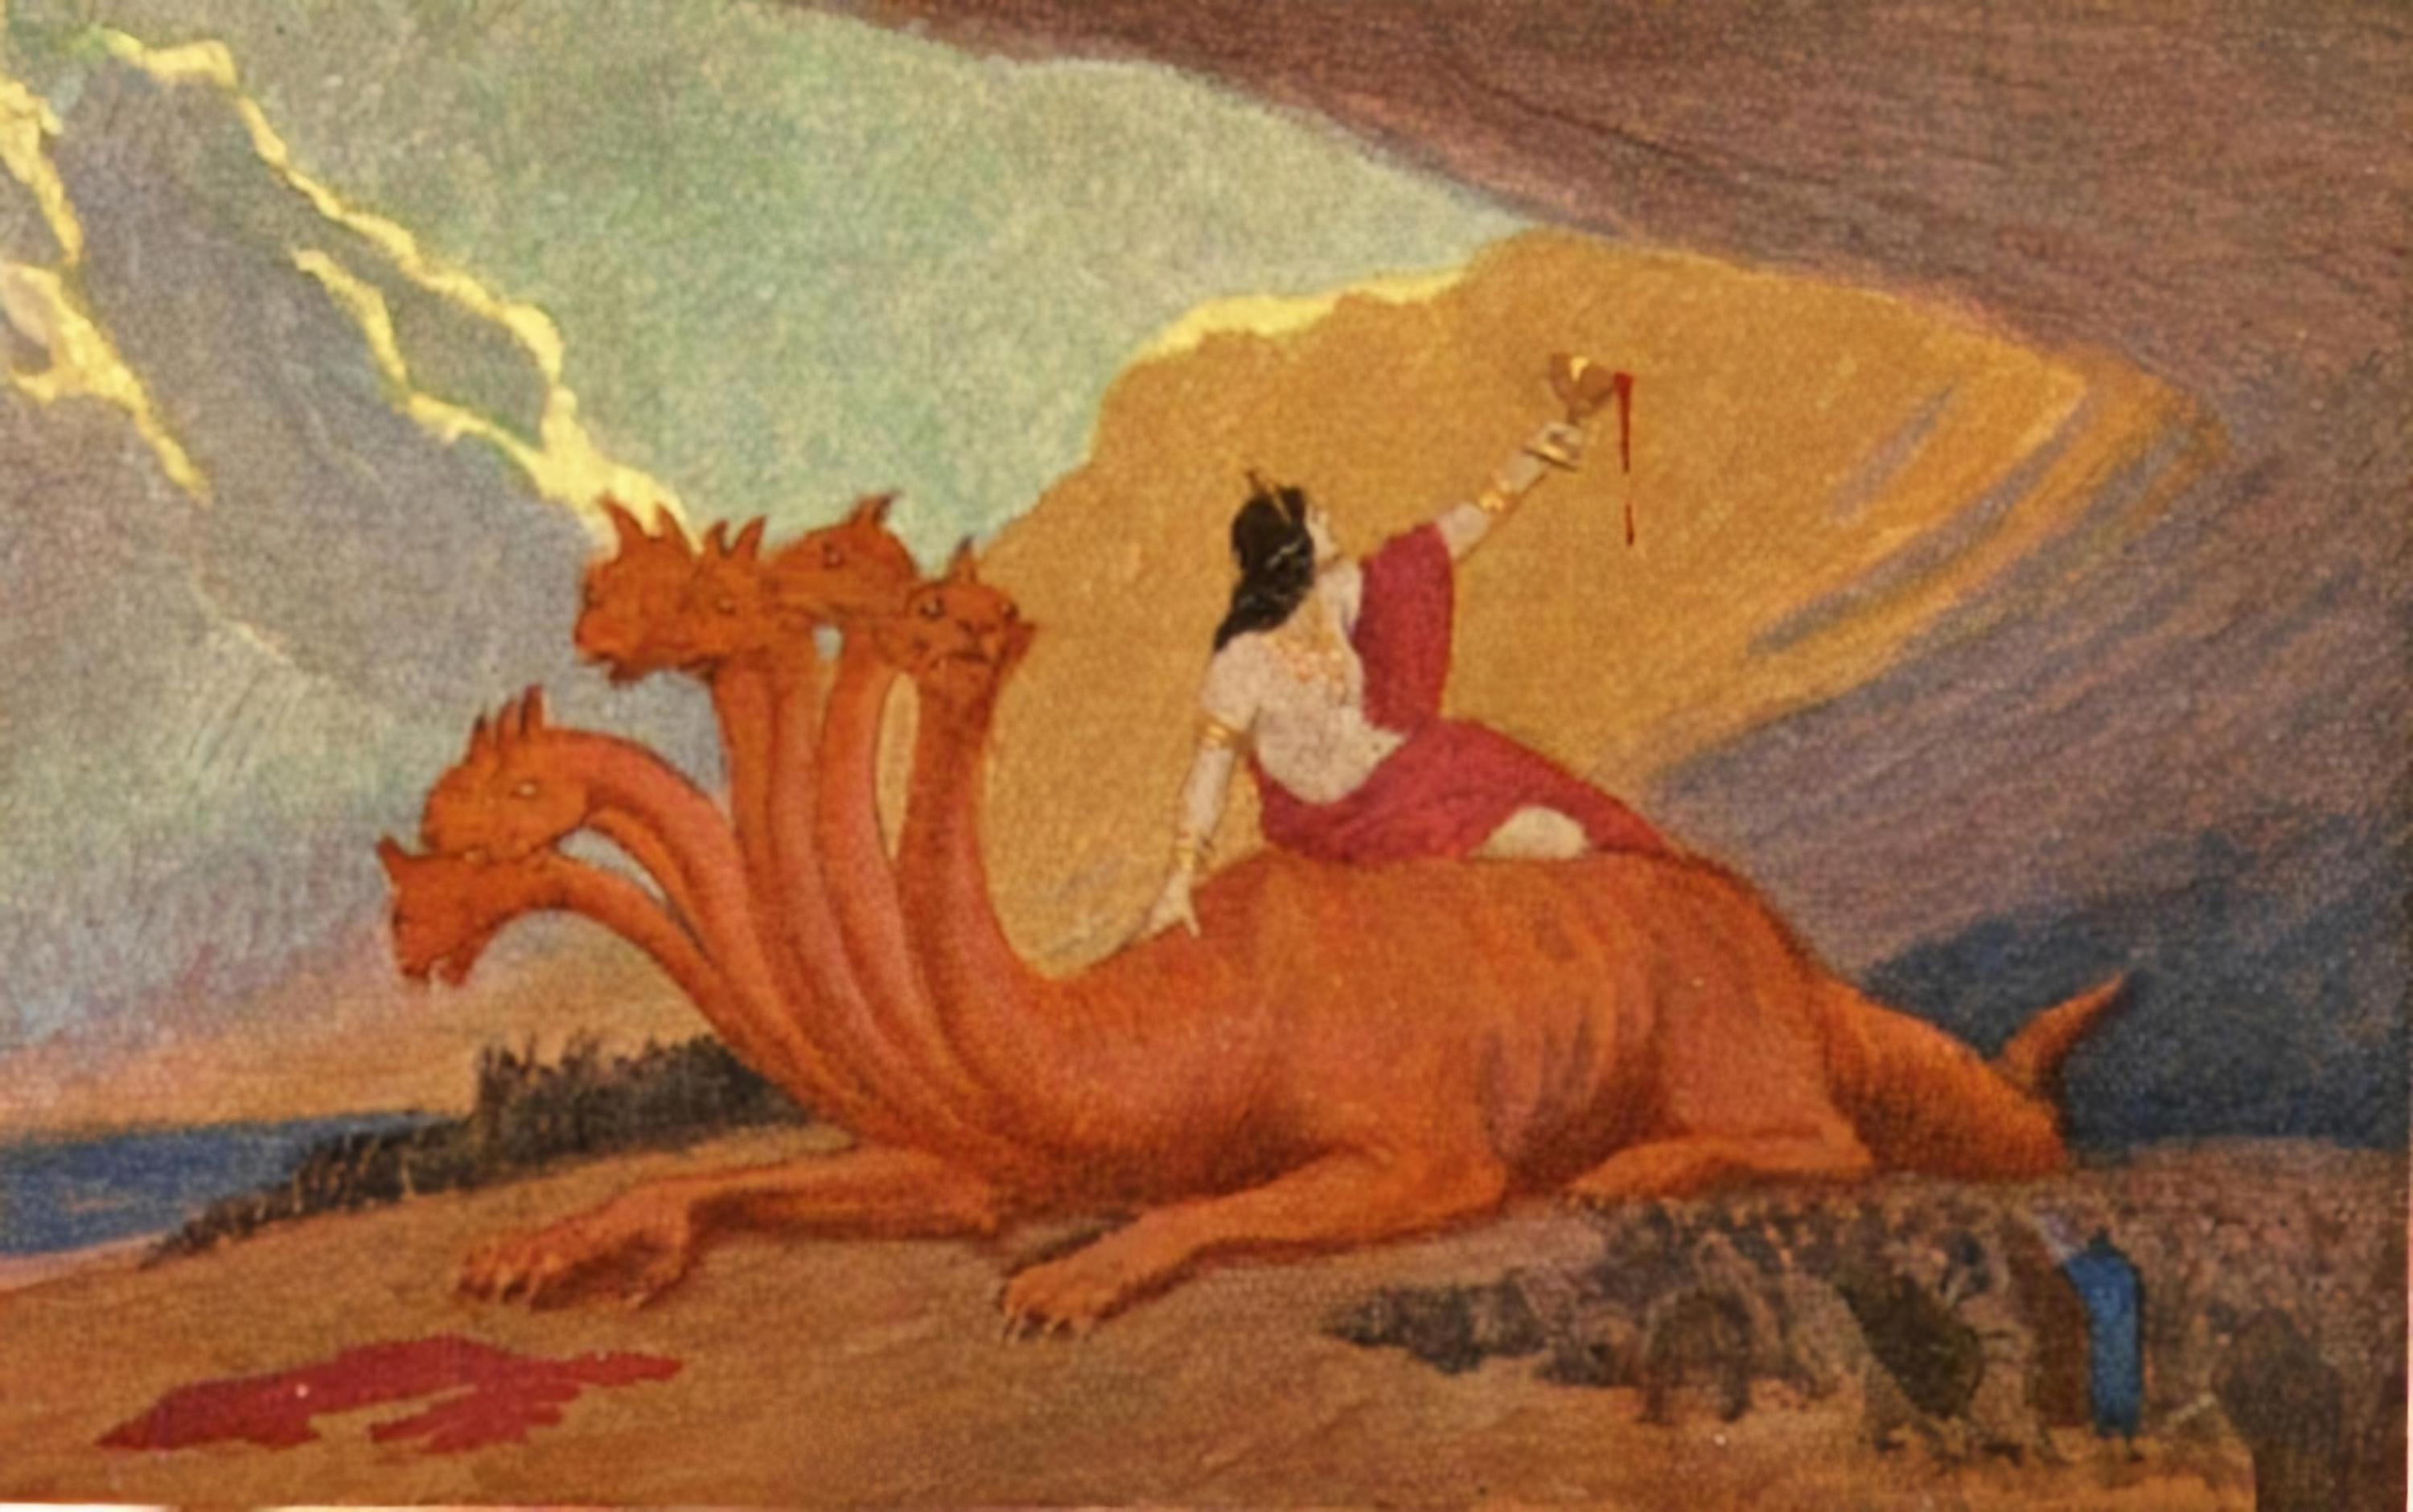
\includegraphics[angle=90, width=0.90\textwidth]{images/illustrations/fugelprostitute}
\end{center}